\chapter{EXPERIMENTAL RESULTS}\nonum

\section{How We Measured}
The numbers come from the Benchmark tab of RenderLab. We ran all five suites once, with 15 timed runs after 5 warm-up runs for every row. The tab reports the median of the timed runs. The exported files are in \texttt{report/data/}, and every number below is copied from them.

\begin{itemize}
\item Computer: a Mac with 10 CPU cores. Browser: headless Chrome 156, driven by a script so the page stayed in focus. A normal browser may give different times.
\item Each frame is 640 by 480 pixels. We ran nothing else during the test.
\item This is one run on one machine. Small differences (a few percent) are not reliable. The comparisons between rows are more useful than the exact milliseconds.
\end{itemize}

\section{Back-Face Culling}
In the demo scene, culling removed 7,757 of the 15,412 triangles (50.33\%). The filled frame took 41.4 ms with culling off and 28.0 ms with it on, which is 1.48 times faster (Table~\ref{tab:cull}). The saving is smaller than the share of culled triangles. Culling still has to move every vertex and adds one test for each triangle. We did not time these parts separately. For the small spheres a frame takes only 1 to 2 ms, and the wireframe differences there (for example 1.125 ms against 1.075 ms) are as small as the noise in the run. We draw no conclusion from those rows.

\begin{table}[H]
\centering
\caption{Frame time with culling off and on (median of 15 runs, ms)}
\label{tab:cull}
\small
\begin{tabular}{@{}lrrrrrr@{}}
\toprule
 & & \multicolumn{3}{c}{Filled} & \multicolumn{2}{c}{Wireframe}\\
\cmidrule(lr){3-5}\cmidrule(l){6-7}
Scene & Culled \% & Off & On & Faster by & Off / on & Faster by\\
\midrule
Reactor scene & 50.33 & 41.4 & 28 & 1.48 & 41.4 / 29.1 & 1.42\\
Sphere, 8 segments & 54.17 & 2.1 & 1.662 & 1.26 & 1.125 / 1.075 & 1.05\\
Sphere, 16 segments & 58.04 & 2.25 & 1.638 & 1.37 & 1.387 / 1.188 & 1.17\\
Sphere, 32 segments & 62.08 & 2.975 & 2 & 1.49 & 2.175 / 1.787 & 1.22\\
Sphere, 64 segments & 62.3 & 5.25 & 3.425 & 1.53 & 4.6 / 3 & 1.53\\
\bottomrule
\end{tabular}
\end{table}

\section{Bresenham against DDA}
We drew 10,000 random lines of three lengths (Table~\ref{tab:line}). Both methods made the same number of pixels, in the same places. DDA was faster in every row, about 1.8 to 2.1 times when drawing. The textbook says Bresenham is faster because it avoids division and decimals, but JavaScript has no separate whole-number type, so every number is already a decimal number and the saving does not appear. Also, our \texttt{bresenhamSteps} stores the error before and after each step so the lab can show a table, so it builds a bigger object for each pixel than DDA does. We did not measure how much of the gap comes from this. The speed benefit of Bresenham is a property of integer hardware, not of this program.

\begin{table}[H]
\centering
\caption{Time for 10,000 lines (median, ms)}
\label{tab:line}
\small
\begin{tabular}{@{}lrrr@{}}
\toprule
Method & Short (10 px) & Medium (100 px) & Long (500 px)\\
\midrule
Bresenham \texttt{drawLine} & 3.2 & 26.5 & 122.5\\
DDA with \texttt{setPixel} & 1.512 & 12.8 & 68\\
\texttt{bresenhamSteps} only & 1.525 & 13 & 83.4\\
\texttt{ddaSteps} only & 0.7438 & 5.9 & 29.2\\
\bottomrule
\end{tabular}
\end{table}

\section{Alpha Compositing}
We applied \texttt{over()} to every pixel of a 640 by 480 image with 1, 2, 4 and 8 layers. The time grows with the number of layers: 4.3 ms for one layer and 25.1 ms for eight, which is 10 to 14 ns per call. For the 3D see-through pass with 6 overlapping panes (432 triangles), the time was 30.4 ms without the sort and 30.8 ms with it. The sort costs about 1.3\%, and it makes the colours correct.

\section{Visvalingam--Whyatt against RDP}
We simplified a seeded coastline of 100 to 2,000 points to 10\% of its points (Table~\ref{tab:vw}). When the number of points doubles, the time of VW grows by about 4 times (4.03 from 500 to 1,000 points and 3.97 from 1,000 to 2,000), which is what $O(n^2)$ predicts. At 2,000 points VW takes 14.3 ms and RDP takes 0.42 ms, so VW is about 34 times slower. This is the cost of our scan for the smallest triangle. For the shape, the two are close. At 500 points the area error is 0.23\% for VW and 0.72\% for RDP, but at 200 points RDP is better (0.31\% against 1.95\%). The largest distance from an original point to the new line was smaller for RDP at every size. So we do not say one method is better on this data.

\begin{table}[H]
\centering
\caption{Simplifying to 10\% of the points (median ms per call)}
\label{tab:vw}
\small
\begin{tabular}{@{}rrrrrr@{}}
\toprule
Points & VW (ms) & VW time ratio & $n^2$ ratio & RDP (ms) & VW area error \%\\
\midrule
100 & 0.04609 & & & 0.009668 & 8.128\\
200 & 0.1508 & 3.271 & 4 & 0.025 & 1.954\\
500 & 0.8938 & 5.927 & 6.25 & 0.07578 & 0.2306\\
1000 & 3.6 & 4.028 & 4 & 0.1734 & 0.0261\\
2000 & 14.3 & 3.972 & 4 & 0.4156 & 0.02659\\
\bottomrule
\end{tabular}
\end{table}

\section{Transformations}
For one million operations each, a \texttt{mat4} multiply took 156 ns and an inverse took 1,047 ns. Turning a point with a quaternion took 12.8 ns and with a matrix 8.6 ns. For these last two rows the minimum (6.5 and 3.7 ns) is far below the median, so they vary between runs. We only say that both are very cheap.

\begin{figure}[H]
\centering
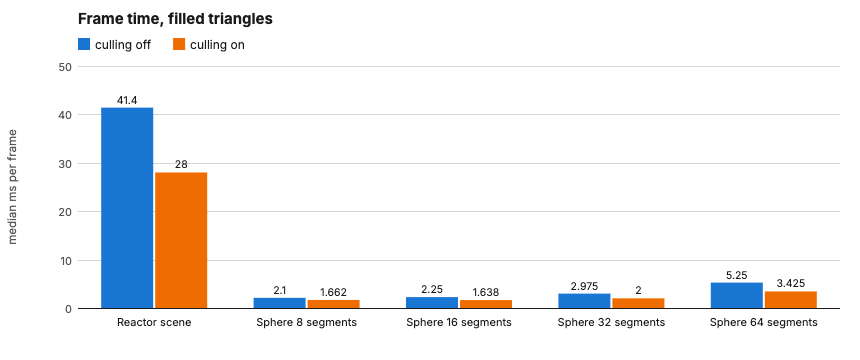
\includegraphics[width=0.48\linewidth]{figures/10-bench-chart-culling.png}\hfill
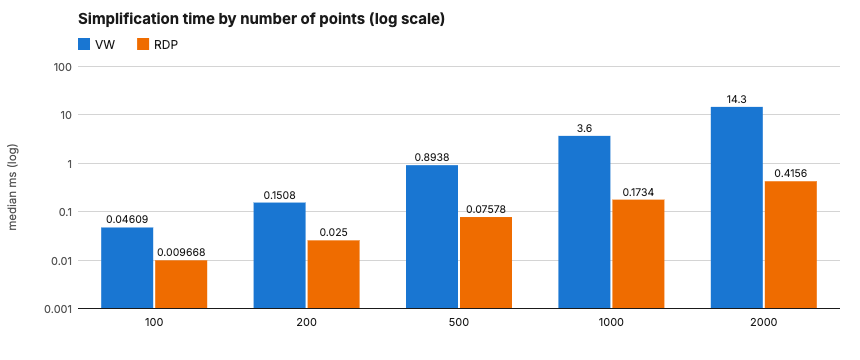
\includegraphics[width=0.48\linewidth]{figures/10-bench-chart-vw.png}
\caption{Charts saved from the Benchmark tab. Left: frame time with culling off and on. Right: time to simplify, VW against RDP.}
\label{fig:benchcharts}
\end{figure}
